\documentclass[a4paper, 14pt]{extarticle}

% Поля
%--------------------------------------
\usepackage{geometry}
\geometry{a4paper,tmargin=2cm,bmargin=2cm,lmargin=3cm,rmargin=1cm}
%--------------------------------------


%Russian-specific packages
%--------------------------------------
\usepackage[T2A]{fontenc}
\usepackage[utf8]{inputenc} 
\usepackage[english, main=russian]{babel}
%--------------------------------------

\usepackage{textcomp}

% Красная строка
%--------------------------------------
\usepackage{indentfirst}               
%--------------------------------------             


%Graphics
%--------------------------------------
\usepackage{graphicx}
\graphicspath{ {./images/} }
\usepackage{wrapfig}
%--------------------------------------

% Полуторный интервал
%--------------------------------------
\linespread{1.3}                    
%--------------------------------------

%Выравнивание и переносы
%--------------------------------------
% Избавляемся от переполнений
\sloppy
% Запрещаем разрыв страницы после первой строки абзаца
\clubpenalty=10000
% Запрещаем разрыв страницы после последней строки абзаца
\widowpenalty=10000
%--------------------------------------

%Списки
\usepackage{enumitem}

%Подписи
\usepackage{caption} 

%Гиперссылки
\usepackage{hyperref}

\hypersetup {
	unicode=true
}

%Рисунки
%--------------------------------------
\DeclareCaptionLabelSeparator*{emdash}{~--- }
\captionsetup[figure]{labelsep=emdash,font=onehalfspacing,position=bottom}
%--------------------------------------

\usepackage{tempora}

%Листинги
%--------------------------------------
\usepackage{listings}
\lstset{
  basicstyle=\ttfamily\footnotesize, 
  %basicstyle=\footnotesize\AnkaCoder,        % the size of the fonts that are used for the code
  breakatwhitespace=false,         % sets if automatic breaks shoulbd only happen at whitespace
  breaklines=true,                 % sets automatic line breaking
  captionpos=t,                    % sets the caption-position to bottom
  inputencoding=utf8,
  frame=single,                    % adds a frame around the code
  keepspaces=true,                 % keeps spaces in text, useful for keeping indentation of code (possibly needs columns=flexible)
  keywordstyle=\bf,       % keyword style
  numbers=left,                    % where to put the line-numbers; possible values are (none, left, right)
  numbersep=5pt,                   % how far the line-numbers are from the code
  xleftmargin=25pt,
  xrightmargin=25pt,
  showspaces=false,                % show spaces everywhere adding particular underscores; it overrides 'showstringspaces'
  showstringspaces=false,          % underline spaces within strings only
  showtabs=false,                  % show tabs within strings adding particular underscores
  stepnumber=1,                    % the step between two line-numbers. If it's 1, each line will be numbered
  tabsize=2,                       % sets default tabsize to 8 spaces
  title=\lstname                   % show the filename of files included with \lstinputlisting; also try caption instead of title
}
%--------------------------------------

%%% Математические пакеты %%%
%--------------------------------------
\usepackage{amsthm,amsfonts,amsmath,amssymb,amscd}  % Математические дополнения от AMS
\usepackage{mathtools}                              % Добавляет окружение multlined
\usepackage[perpage]{footmisc}
%--------------------------------------

%--------------------------------------
%			НАЧАЛО ДОКУМЕНТА
%--------------------------------------

\begin{document}

%--------------------------------------
%			ТИТУЛЬНЫЙ ЛИСТ
%--------------------------------------
\begin{titlepage}
\thispagestyle{empty}
\newpage


%Шапка титульного листа
%--------------------------------------
\vspace*{-60pt}
\hspace{-65pt}
\begin{minipage}{0.3\textwidth}
\hspace*{-20pt}\centering

\includegraphics[width=\textwidth]{emblem}
\end{minipage}
\begin{minipage}{0.67\textwidth}\small \textbf{
\vspace*{-0.7ex}
\hspace*{-6pt}\centerline{Министерство науки и высшего образования Российской Федерации}
\vspace*{-0.7ex}
\centerline{Федеральное государственное бюджетное образовательное учреждение }
\vspace*{-0.7ex}
\centerline{высшего образования}
\vspace*{-0.7ex}
\centerline{<<Московский государственный технический университет}
\vspace*{-0.7ex}
\centerline{имени Н.Э. Баумана}
\vspace*{-0.7ex}
\centerline{(национальный исследовательский университет)>>}
\vspace*{-0.7ex}
\centerline{(МГТУ им. Н.Э. Баумана)}}
\end{minipage}
%--------------------------------------

%Полосы
%--------------------------------------
\vspace{-25pt}
\hspace{-35pt}\rule{\textwidth}{2.3pt}

\vspace*{-20.3pt}
\hspace{-35pt}\rule{\textwidth}{0.4pt}
%--------------------------------------

\vspace{1.5ex}
\hspace{-35pt} \noindent \small ФАКУЛЬТЕТ\hspace{80pt} <<Информатика и системы управления>>

\vspace*{-16pt}
\hspace{47pt}\rule{0.83\textwidth}{0.4pt}

\vspace{0.5ex}
\hspace{-35pt} \noindent \small КАФЕДРА\hspace{50pt} <<Теоретическая информатика и компьютерные технологии>>

\vspace*{-16pt}
\hspace{30pt}\rule{0.866\textwidth}{0.4pt}
  
\vspace{11em}

\begin{center}
\Large {\bf Лабораторная работа № 1} \\ 
\large {\bf по курсу <<Компьютерные сети>>} \\
\large <<web-сервера>> 
\end{center}\normalsize

\vspace{8em}


\begin{flushright}
  {Студент группы ИУ9-32Б Волохов А. В. \hspace*{15pt}\\ 
  \vspace{2ex}
  Преподаватель Посевин Д. П.\hspace*{15pt}}
\end{flushright}

\bigskip

\vfill
 

\begin{center}
\textsl{Москва 2023}
\end{center}
\end{titlepage}
%--------------------------------------
%		КОНЕЦ ТИТУЛЬНОГО ЛИСТА
%--------------------------------------

\renewcommand{\ttdefault}{pcr}

\setlength{\tabcolsep}{3pt}
\newpage
\setcounter{page}{2}

\section{Задание}\label{Sect::task}
Рассматривается задача разработки web-сервера на языке GO на основе пакета net/http. 
Необходимо:
\begin{itemize}
\item Реализовать web-сервер и запустить на заданном порте.
\item Изучить принимаемые web-сервером параметры, реализовать передачу данных методом РОST. Вывести значения введенные в форму
\item Реализовать вывод форматированного гипертекста с контекстным меню в виде гиперссылок, при клике на гиперссылку должна выполняться подмена контента;
\end{itemize}
Далее рассматривается задача разработки приложения на языке GO реализующего синтаксический разбор XML файла формата RSS. 
Необходимо Реализовать получение данных из различных RSS- каналов по вариантам. Сравнить результаты разбора и сделать выводы.
В итоге необходимо разработать web-сервер, который выполняет соединение с удаленным (удаленными) серверами RSS-новостей и возвращает результаты обработки данных в структурированном виде (страница гипертекста) web-клиенту, в нашем случае в браузер по вариантам.
\section{Результаты}\label{Sect::res}

Исходный код программы представлен в листингах~\ref{lst:code1}--~\ref{lst:code2}--~\ref{lst:code3}.

\begin{figure}[!htb]
\begin{lstlisting}[language={Go},caption={o.1.go},label={lst:code1}]
package main

import (
	"fmt"
	"html/template"
	"io/ioutil"
	"net/http"
	"sync"
)

var data struct {
	Name string
	Age  string
}

var mutex sync.Mutex

func FormHandler(w http.ResponseWriter, r *http.Request) {
	if r.Method == http.MethodPost {
		name := r.FormValue("name")
		age := r.FormValue("age")

		mutex.Lock()
		data.Name = name
		data.Age = age
		mutex.Unlock()

		http.Redirect(w, r, "/data", http.StatusSeeOther)
		return
	}

	w.Header().Set("Content-Type", "text/html")
	http.ServeFile(w, r, "/home/alex/BMSTU_git/IU9-CN-GO/lab1/0.1/form.html")
}

func DataHandler(w http.ResponseWriter, r *http.Request) {
	mutex.Lock()
	defer mutex.Unlock()
\end{lstlisting}
\end{figure}

\newpage

\begin{figure}[!htb]
\begin{lstlisting}[language={Go},caption={o.1.go - продолжение},label={lst:code2}]
	htmlContent, err := ioutil.ReadFile("/home/alex/BMSTU_git/IU9-CN-GO/lab1/0.1/data.html")
	if err != nil {
		http.Error(w, "Internal Server Error", http.StatusInternalServerError)
		return
	}

	tmpl, err := template.New("data").Parse(string(htmlContent))
	if err != nil {
		http.Error(w, "Internal Server Error", http.StatusInternalServerError)
		return
	}

	w.Header().Set("Content-Type", "text/html")
	err = tmpl.Execute(w, data)
	if err != nil {
		http.Error(w, "Internal Server Error", http.StatusInternalServerError)
		return
	}
}

func main() {
	http.HandleFunc("/", FormHandler)
	http.HandleFunc("/data", DataHandler)

	err := http.ListenAndServe(":9000", nil)
	if err != nil {
		fmt.Println("Server error:", err)
	}
}
\end{lstlisting}
\end{figure}

\newpage
\begin{figure}[!htb]
\begin{lstlisting}[language={HTML},caption={form.html},label={lst:code3}]
<!DOCTYPE html>
<html lang="en">
<head>
  <meta charset="UTF-8">
  <title>Form</title>
</head>
<body>
<h1>Enter the data:</h1>
<form action="/" method="post">
  <label for="name">Name:</label>
  <input type="text" id="name" name="name"><br><br>

  <label for="age">Age:</label>
  <input type="text" id="age" name="age"><br><br>

  <input type="submit" value="Send">
</form>
</body>
</html>
\end{lstlisting}
\end{figure}
\newpage
\begin{figure}[!htb]
\begin{lstlisting}[language={HTML},caption={data.html},label={lst:code4}]
<!DOCTYPE html>
<html lang="en">
<head>
    <meta charset="UTF-8">
    <title>Form data</title>
</head>
<body>
<h1>Form data:</h1>
<p>Name: {{.Name}}</p>
<p>Age: {{.Age}}</p>
</body>
</html>

\end{lstlisting}
\end{figure}
\newpage
\begin{figure}[!htb]
\begin{lstlisting}[language={Go},caption={o.2.go},label={lst:code5}]
package main

import (
	"fmt"
	"github.com/mmcdole/gofeed"
	"log"
)

func main() {
	fp := gofeed.NewParser()

	rssUrls := []string{
		"https://vesti-k.ru/rss/",
	}

	for _, url := range rssUrls {
		feed, err := fp.ParseURL(url)
		if err != nil {
			log.Fatalf("Error parsing RSS from URL %s: %v\n", url, err)
		}

		fmt.Printf("Title : %s\n", feed.Title)
		fmt.Printf("Description : %s\n", feed.Description)
		fmt.Printf("Number of Items : %d\n", len(feed.Items))

		for i, item := range feed.Items {
			fmt.Println()
			fmt.Printf("Item Number : %d\n", i)
			fmt.Printf("Title : %s\n", item.Title)
			fmt.Printf("Link : %s\n", item.Link)
			fmt.Printf("Description : %s\n", item.Description)
			fmt.Printf("Published Date : %s\n", item.Published)
		}
	}
}
\end{lstlisting}
\end{figure}

\newpage

\begin{figure}[!htb]
\begin{lstlisting}[language={Go},caption={o.3.go},label={lst:code6}]
package main

import (
	"fmt"
	"github.com/mmcdole/gofeed"
	"html/template"
	"net/http"
	"sync"
)

var data struct {
	RssUrl string
}

var mutex sync.Mutex

func FormHandler(w http.ResponseWriter, r *http.Request) {
	if r.Method == http.MethodPost {
		rssUrl := r.FormValue("rssUrl")

		mutex.Lock()
		data.RssUrl = rssUrl
		mutex.Unlock()

		http.Redirect(w, r, "/news", http.StatusSeeOther)
		return
	}

	w.Header().Set("Content-Type", "text/html")
	http.ServeFile(w, r, "/home/alex/BMSTU_git/IU9-CN-GO/lab1/0.3/form.html")
}

func NewsHandler(w http.ResponseWriter, r *http.Request) {
	mutex.Lock()
	rssUrl := data.RssUrl
	mutex.Unlock()

	fp := gofeed.NewParser()
	feed, err := fp.ParseURL(rssUrl)
	if err != nil {
		http.Error(w, "Error parsing RSS feed", http.StatusInternalServerError)
		return
	}

\end{lstlisting}
\end{figure}

\newpage
\begin{figure}[!htb]
\begin{lstlisting}[language={Go},caption={o.3.go - продолжение},label={lst:code7}]

	tmpl, err := template.ParseFiles("/home/alex/BMSTU_git/IU9-CN-GO/lab1/0.3/news.html")
	if err != nil {
		http.Error(w, "Error loading template", http.StatusInternalServerError)
		return
	}

	w.Header().Set("Content-Type", "text/html")
	err = tmpl.Execute(w, feed)
	if err != nil {
		http.Error(w, "Error executing template", http.StatusInternalServerError)
		return
	}
}

func main() {
	http.HandleFunc("/", FormHandler)
	http.HandleFunc("/news", NewsHandler)

	err := http.ListenAndServe(":9000", nil)
	if err != nil {
		fmt.Println("Server error:", err)
	}
}
\end{lstlisting}
\end{figure}

\newpage
\begin{figure}[!htb]
\begin{lstlisting}[language={HTML},caption={form.html},label={lst:code8}]
<!DOCTYPE html>
<html lang="en">
<head>
    <meta charset="UTF-8">
    <title>Entering an RSS Feed</title>
</head>
<body>
<h1>Enter RSS Feed URL</h1>
<form action="/parse" method="post">
    <label for="rssUrl">RSS feed URL:</label>
    <input type="text" id="rssUrl" name="rssUrl" required>
    <input type="submit" value="Send">
</form>
</body>
</html>
\end{lstlisting}
\end{figure}

\newpage
\begin{figure}[!htb]
\begin{lstlisting}[language={HTML},caption={news.html},label={lst:code9}]
<!DOCTYPE html>
<html lang="en">
<head>
  <meta charset="UTF-8">
  <title>Links to news</title>
</head>
<body>
<h1>Links to news:</h1>
<ul>
  {{range .Items}}
  <li><a href="{{.Link}}">{{.Title}}</a></li>
  {{end}}
</ul>
</body>
</html>
\end{lstlisting}
\end{figure}



\begin{figure}[!htb]
	\centering
	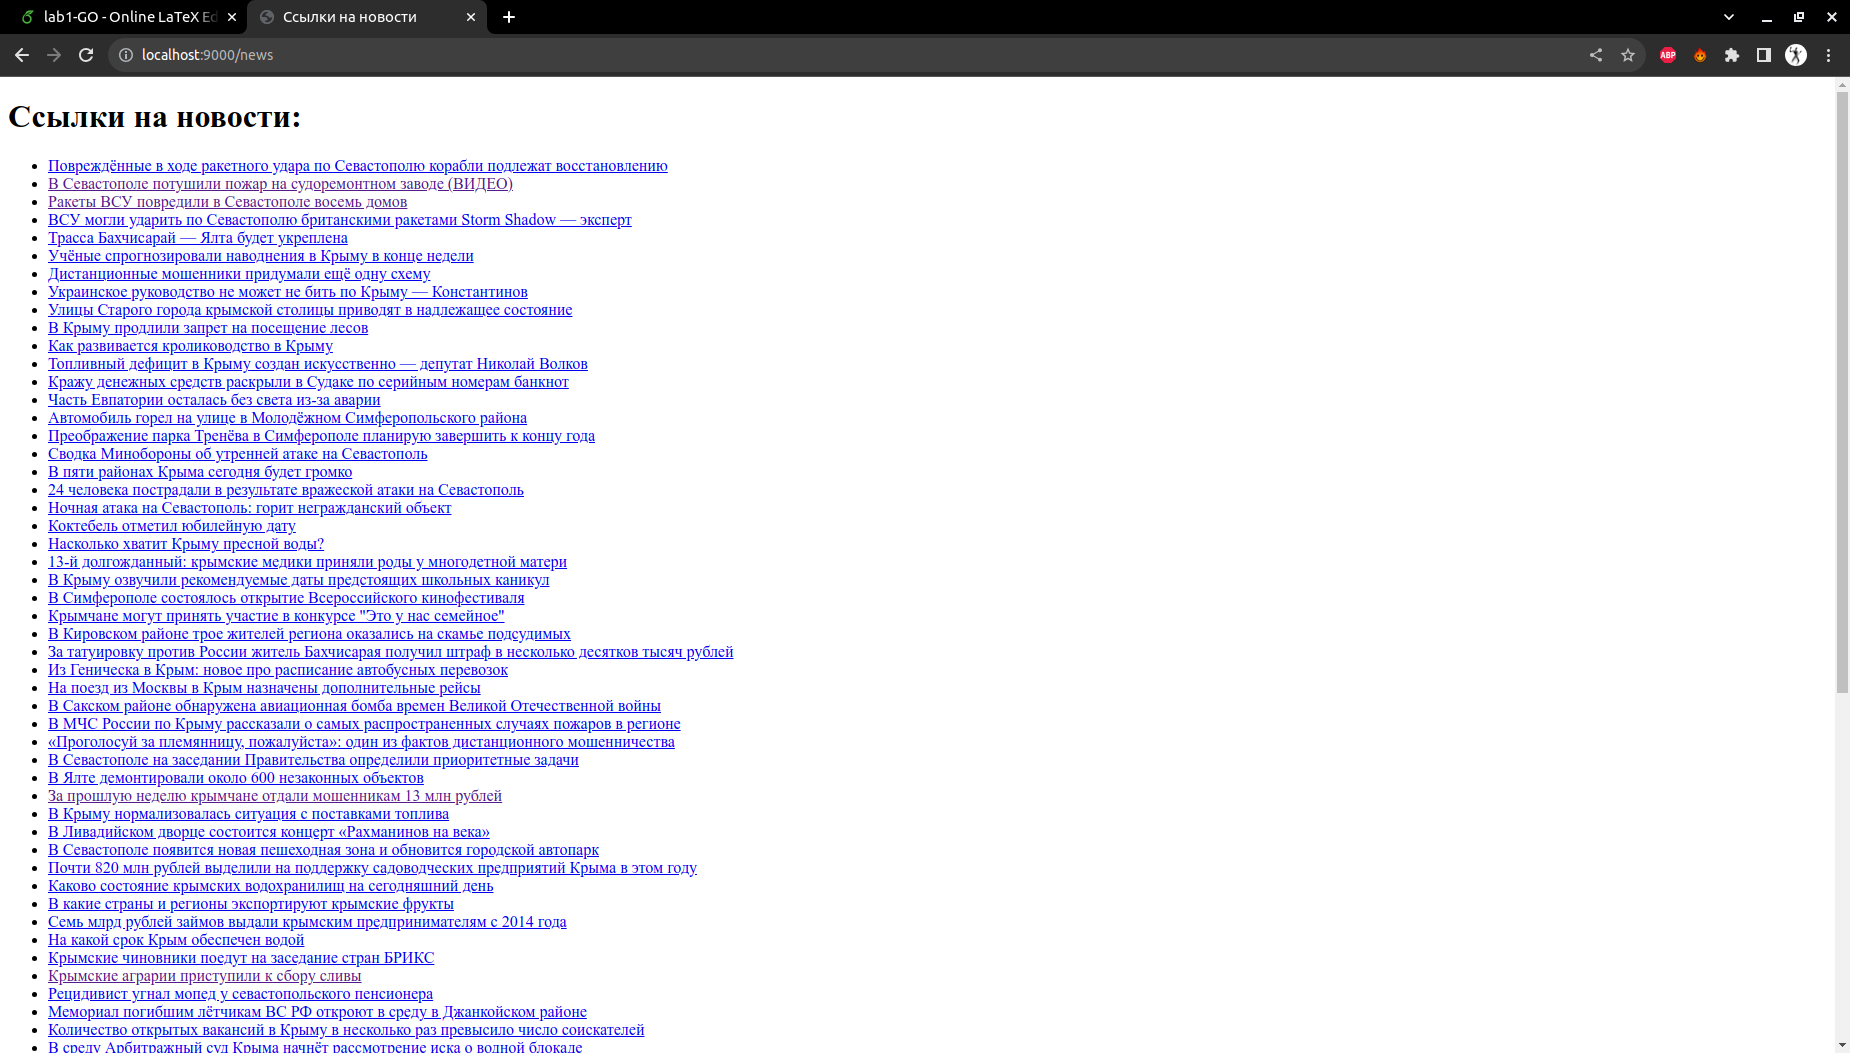
\includegraphics[width=0.8\textwidth]{result.png}
\caption{Результат}
\label{fig:img1}
\end{figure}





\end{document}